\documentclass{report}
\usepackage{graphicx}
\usepackage{appendix}
\usepackage{pdfpages}
\title{HARE: Final Report}
\author{Sandia National Labs, IBM, Bell Labs, Vita Nuova
\thanks{\protect
\includegraphics[height=0.3in]{thunderchicken}
}
\thanks{\protect

\includegraphics[height=0.3in]{DOELOGO}%
}%
\thanks{Sandia National Laboratories is a multi-program laboratory managed and operated by Sandia Corporation, a wholly owned subsidiary of Lockheed Martin Corporation, for the U.S. Department of Energy’s National Nuclear Security Administration under contract DE-AC04-94AL85000. SAND- 2011-xxxxC.}  
}
\date{\today}

\begin{document}
\maketitle
\tableofcontents
\pagebreak

This report documents the results of work done over a 6 year period under the FAST-OS 
programs. The first effort was called Right-Weight Kernels, (RWK) and was concerned with 
improving measurements of OS noise so it could be treated quantitatively; 
and evaluating the use of two operating systems, Linux
and Plan~9, on HPC systems and determining how these operating systems needed
to be extended or changed for HPC, while still retaining their general-purpose nature. 

The second program, HARE, explored the creation of alternative runtime models, 
building on RWK. All of the HARE work was done on Plan~9. The HARE reseachers
were mindful of the very good Linux and LWK work being done at other labs and saw no
need to recreate it. 

The organizations included LANL (RWK) and Sandia (RWK, HARE), as the PI moved to Sandia; 
IBM; Bell Labs; and Vita Nuova, as a subcontractor to Bell Labs. In any given year, 
the funding was suffcient to cover a PI from each organization part time. 

Even given this limited funding, the two efforts had outsized impact: 
\begin{itemize}
\item Helped Cray decide to use Linux, instead of a custom kernel, and provided
the tools needed to make Linux perform well
\item Created a successor operating system to Plan~9, NIX, which has been taken in 
by Bell Labs for further development
\item Created a standard system measurement tool, Fixed Time Quantum or FTQ, which is widely
used for measuring operating systems impact on applications
\item Spurred the use of the 9p protocol in several organizations, including IBM
\item Built software in use at many companies, including IBM, Cray, and Google
\item Spurred the creation of alternative runtimes for use on HPC systems
\item Demonstrated that, with proper modifications, a general purpose operating systems
can provide communications up to 3 times as effective as user-level libraries
\end{itemize}

Open source was a key part of this work. The code developed for this project 
is in wide use and available at many places. The core Blue Gene code is 
available at https://bitbucket.org/ericvh/hare. 

We describe details of these impacts in the following sections. The rest of this 
report is organized as follows: first, we describe commercial impact; next, 
we describe the FTQ benchmark and its impact in more detail; operating systems
and runtime research follows; we discuss infrastructure software; and close with a 
description of the new NIX  operating system, future work, and conclusions. 
\chapter{Commercial Impact}
\section{Cray}
In August 2006, we had meetings with Cray to explore the use of Linux on their supercomputers 
in place of the Light Weight Kernel then shipping. The discussions aligned with the 
basic thesis of our Right Weight Kernel project, which was that a properly designed 
subset of a commercial kernel, coupled with a set of carefully designed extensions, could 
compete with Light Weight Kernels, in additon to bringing in the advantages of a more
standard programming environment. 

Larry Kaplan, of Cray, notes: ``The FastOS forums sponsored by the DOE
Office of Science were a very important part of Cray's investigations
into compute node operating systems for HPC.  The Right Weight Kernel
project in particular provided important information on the challenges
of using Linux which helped drive the research and development done at
Cray in order to deliver the Cray Linux Environment.  Cray fully
believes in the importance of the research community and the ability
for them to help influence our direction and success and looks forward
to future opportunities for collaboration.''

As part of Right Weight Kernel project, we created the Fixed Time
Quantum\cite{ftq} benchmark in order to support quantitative
evaluation of OS noise. Cray used this benchmark to evaluate and
improve the performance of their Compute Node Linux
product\cite{kaplan2007cray}.


\section{IBM}
IBM Research's involvement in this project has been extremely valuable in exploring
ways to broaden the applicability of the BlueGene hardware through alternative software
stacks.  It has allowed us to explore hardware features which aren't used by the production
software as well as explore alternative schemes for scalability and reliability which are
difficult or impossible under the production software.  This alternative view has given us
new insights which can then be incorporated into future hardware designs as well as future
production system software.

IBM also used FTQ to instrument the Blue Gene kernel\cite{bgpftq}.

\subsection{9p}

Our involvement in the HARE project has increased the visibility and use
of the Plan 9 resource sharing protocol, known as 9p, within the broader IBM community.
In particular, during the course of the HARE project we incorporated both 9p and the XCPU
workload management system into a hybrid computing platform called the Virtual Power
Environment~\cite{VPE}, which was developed for the Marenustrum supercomputer at the Barcelona 
Supercomputing Center.  Infrastructures derrived from the original VPE idea are still
under development by HPC Links under the product named VERTEX~\cite{vertex}.
Experiences from the VPE effort were factored back into XCPU
resulting in the creation of the XCPU2~\cite{xcpu2} workload mangaement framework which then was
factored back into the HARE project as XCPU3~\cite{xcpu3} and the 
Unified Execution Model~\cite{uem}.  The fundamental components, Linux kernel support, and
advanced XCPU models were all developed as a direct result of the HARE funding.

Outside of the high performance computing area, the 9p protocol has achieved great success
within the emerging virtualization and cloud computing area as the defacto cloud computing
paravirtualized file system under Linux.  In coordination with IBM Research, development
teams have created a virtio~\cite{virtio} transport for 9p and incorporated a 9p server into
Qemu~\cite{qemu} which allows any KVM machines to be able to directly mount file systems
from the host~\cite{virtfs}.  This technology has been part of the main line kernel for about
a year and is being incorporated into the commercial Linux distributions.

\subsection{Hybrid Kernels}

Additionally, our experiences with hybrid environments on BlueGene with different kernel
types running on different nodes has led us towards a hybrid kernel model for future
massive multicore platforms where we are looking at taking advantage of running different
types of kernels on different cores in order to improve performance and efficiency by
insulating application cores from operating system noise.  These so called "hybrid" kernels
are currently being evaluated to be the default production kernel on future platforms.

\subsection{Analytics}

Several of the workload distribution methodologies we explored 
during the HARE project are also being evaluated for use in large-scale
analytics systems.  In particular, the unified execution model and PUSH~\cite{PUSH}
workflow are being looked at for application within analytics clusters as an alternative to
Hadoop for certain scenarios and the multipipe technology developed as part of HARE is
also being evaluated for integration into several internal projects.

In addition to workflow management, IBM is also exploring the application of
9p synthetic and static file system technologies to analytics file systems which
can be used with our execution model or with more conventional analytics software
such as Hadoop. 

\section{Coraid}
Coraid is a fast-growing vendor of network disk systems used in cloud computing centers. 
Coraid uses the trace software we developed\cite{plan9trace} for Blue Gene. 
This software extends both the kernel and the linker to enable convenient, efficient 
performance tracing of kernel functions. A measure of the efficiency of this software 
is that  all of Coraid's production
kernels ship with the tracing software always installed and enabled. 
The capability provided by the software is so useful, and the performance impact so small, 
that Coraid decided that it should always be available. 

\section{Google}
As a first step in the FAST-OS project, in 2005 we 
funded the creation of  a compiler toolchain (C compiler, linker, and assembler) for Plan 9 on the 
AMD/Intel 64-bit architectures, known as Opteron and EM64-T.
As per a basic requirement of the project, these
tools were created as open source. 

Google has recently released a new programming language called Go. Go supports, among other 
architectures, the AMD/Intel 64-bit CPUs. For these CPUs, Google adapted the  Plan 9 C toolchain
we created. There is hence a very direct link from the FAST-OS funding to Google's Go programming 
language, a language which is seeing very wide adoption. 

\chapter{Fixed Time Quantum}

Fixed Time Quantum\cite{ftq} is a tool for creating measurements of operating system noise, allowing users to do quantitative analysis 
with
standard tools such as Matlab and GNU Octave.

FTQ has found wide use in both the research and commercial world, having become one of the standard measurement tools for OS noise. 
Both IBM and Cray have used it to help tune their operating system kernels for minimal noise. 
FTQ results supported Cray's decision to move to Compute Node Linux, replacing the Catamount Light Weight Kernel originally delivered with those systems. Real 
application results supported the initial results from FTQ. 

The distinguishing feature of FTQ is that it measures work per fixed amount of time, rather than the more traditional time taken to do a fixed amount of work. The distinction is subtle but essential.  FTQ is written to carefully ensure that the time samples are for a fixed amount but also that the sampling interval is {\em stationary}. FTQ ensures this property by starting each sample interval at the correct point in time even if, due to interference, the previous sample interval took too long. For more discussion of how this is done the reader is referred to the original paper. 

As mentioned, FTQ allows users and vendors to use quantitative, rather than qualitative analysis.  As an example we will walk through real data taken on 
Blue Gene/P on a very early implementation of Plan 9. 
The FTQ program produces two output files: a so-called "counts" file, and a times file. These two files allow a user to reconstruct how much work was done per interval. The files 
are useful independent of each other: the counts data gives some idea of how much work was done, so
that the same binary, under different operating system, can compare how well the applications run.
The times data can be used to determine how well the algorithm that maintains stationary sampling is
doing its job; deviations of the time from a desired baseline can point to operating system, virtual
machine,  or even hardware problems: the times file was used to diagnose virtual machine interference on the Purple system at LLNL. Combined, the two files can be used for deeper analysis, combining both work and time information. 

While the raw data is useful, it is possible to misread too much into a raw data plot. In the original paper we showed two traces, one of them generated by white noise and the other by a very well-defined signal. To the naked eye, they are indistinguishable. Further processing of the data is essential to ensure that the measured data represents information, not white noise. 

In Figure \ref{rawdata}, we show a similar plot for three FTQ runs, on CNK, Linux, and Plan 9. What is of interest are not the actual numbers -- the Plan~9 binary 
is a different binary -- but the occurrence of spikes in the graph. One can gain some information immediately: there is clearly periodic interference of the same 
frequency for each operating system. Further investigation revealed that the 64-bit processor clock, comprised of two 32-bit counters, had a glitch when the
low-order 32-bit counter rolled over, leading to a slightly longer sample interval at that point. The algorithm quickly resynchronized, however, such that the 
counts over a long period were correct. This spike can easily be misinterpreted in the time domain graph; it does not have any impact on the frequency domain graph. 
\begin{figure}[h]
\begin{center}
 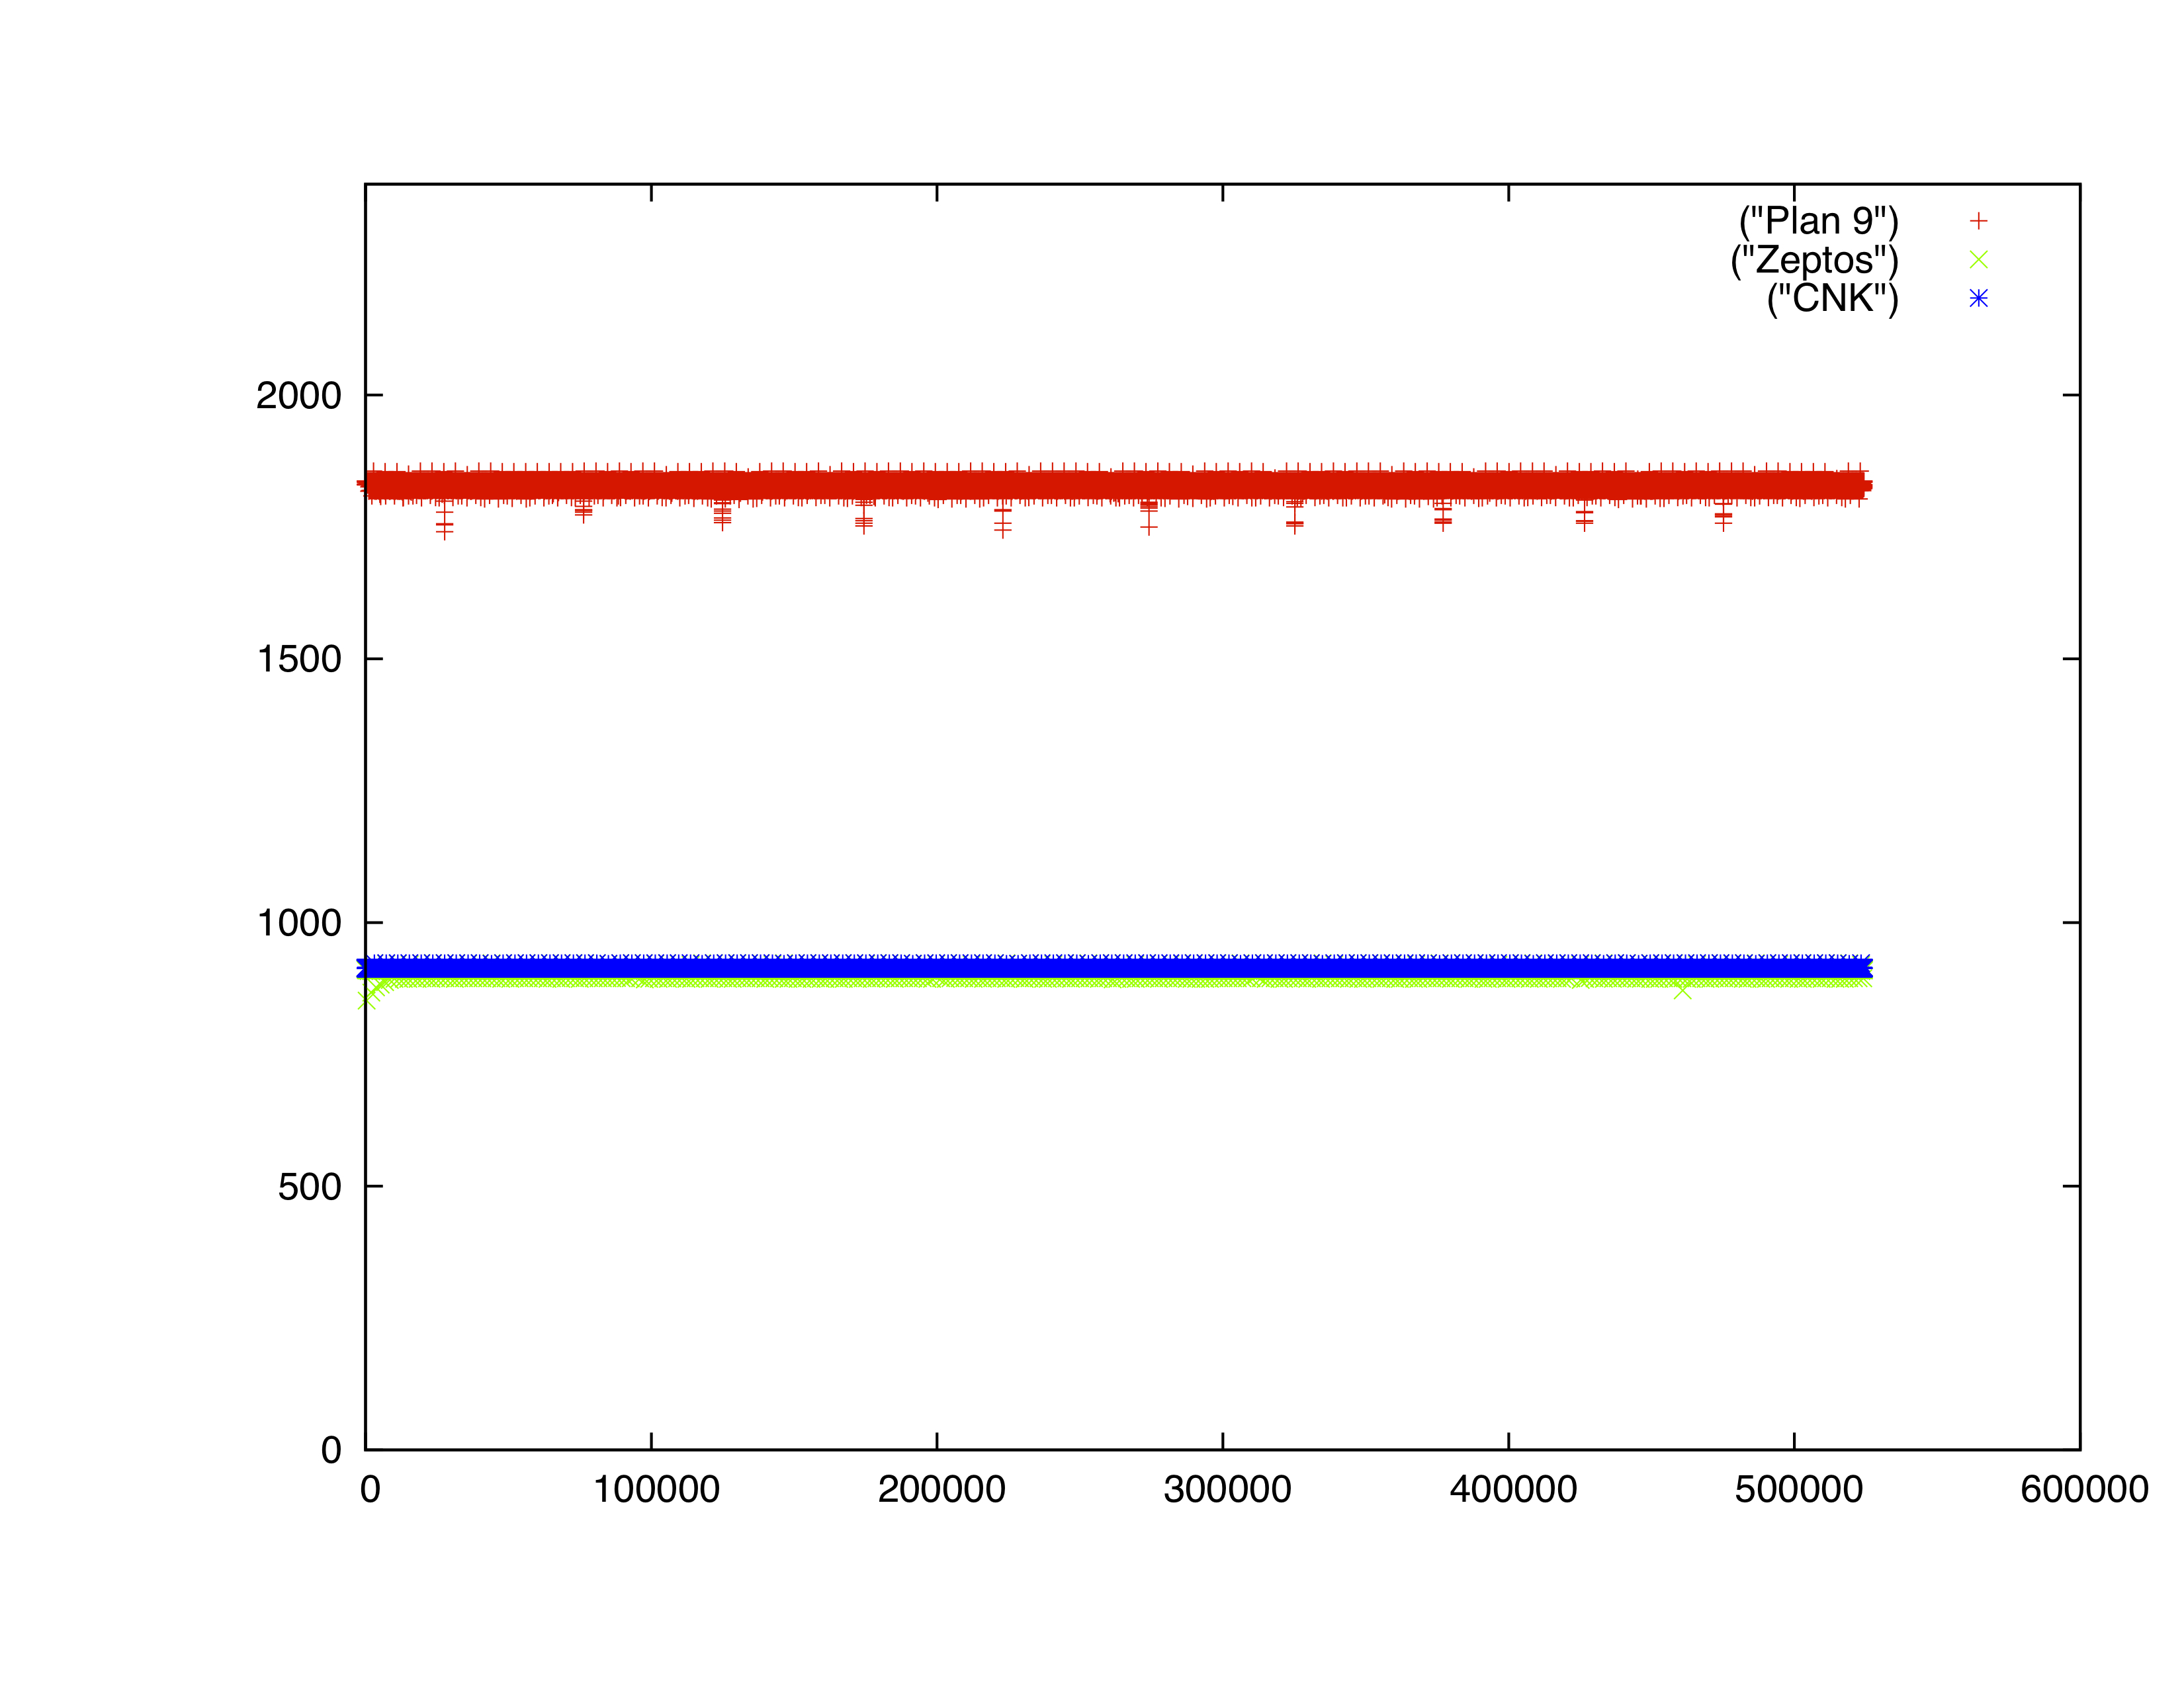
\includegraphics[width=4in]{raw.jpg}
 \caption{{\bf A plot of FTQ 'count' data for three Blue Gene/P operating systems, with sample
 number on the X axis and unit-less work on the Y axis.}}
\label{rawdata}
\end{center}
\end{figure}

Converting this data to the fequency domain is relatively straightforward. We present the octave script in Figure \ref{octave}. 
\begin{figure}[h]
\begin{center}
\begin{verbatim}
samples = readcounts('9ftq63_0_counts.dat');
samples = fitmax(samples);
[Psd,w] = pwelch(samples,[],[],[],810);
\end{verbatim}
\caption{Octave script for processing raw FTQ data. We only use the counts file in this case.}
\label{octave}
\end{center}
\end{figure}
The program reads the file in using a function that returns a one-dimensional vector. The function
{\tt fitmax} normalizes all the values in the vector to the maximum value. Finally, 
the code calls the octave pwelch function, which generates two vectors: a power spectrum estimation (Psd) and a set of frequencies(w). The parameters are the samples, and the 
cycle counter 
frequency (810 Mhz.). 
We show a plot of the Power spectral density for the three operating systems in Figure \ref{psd}
\begin{figure}[htbp]
\begin{center}
 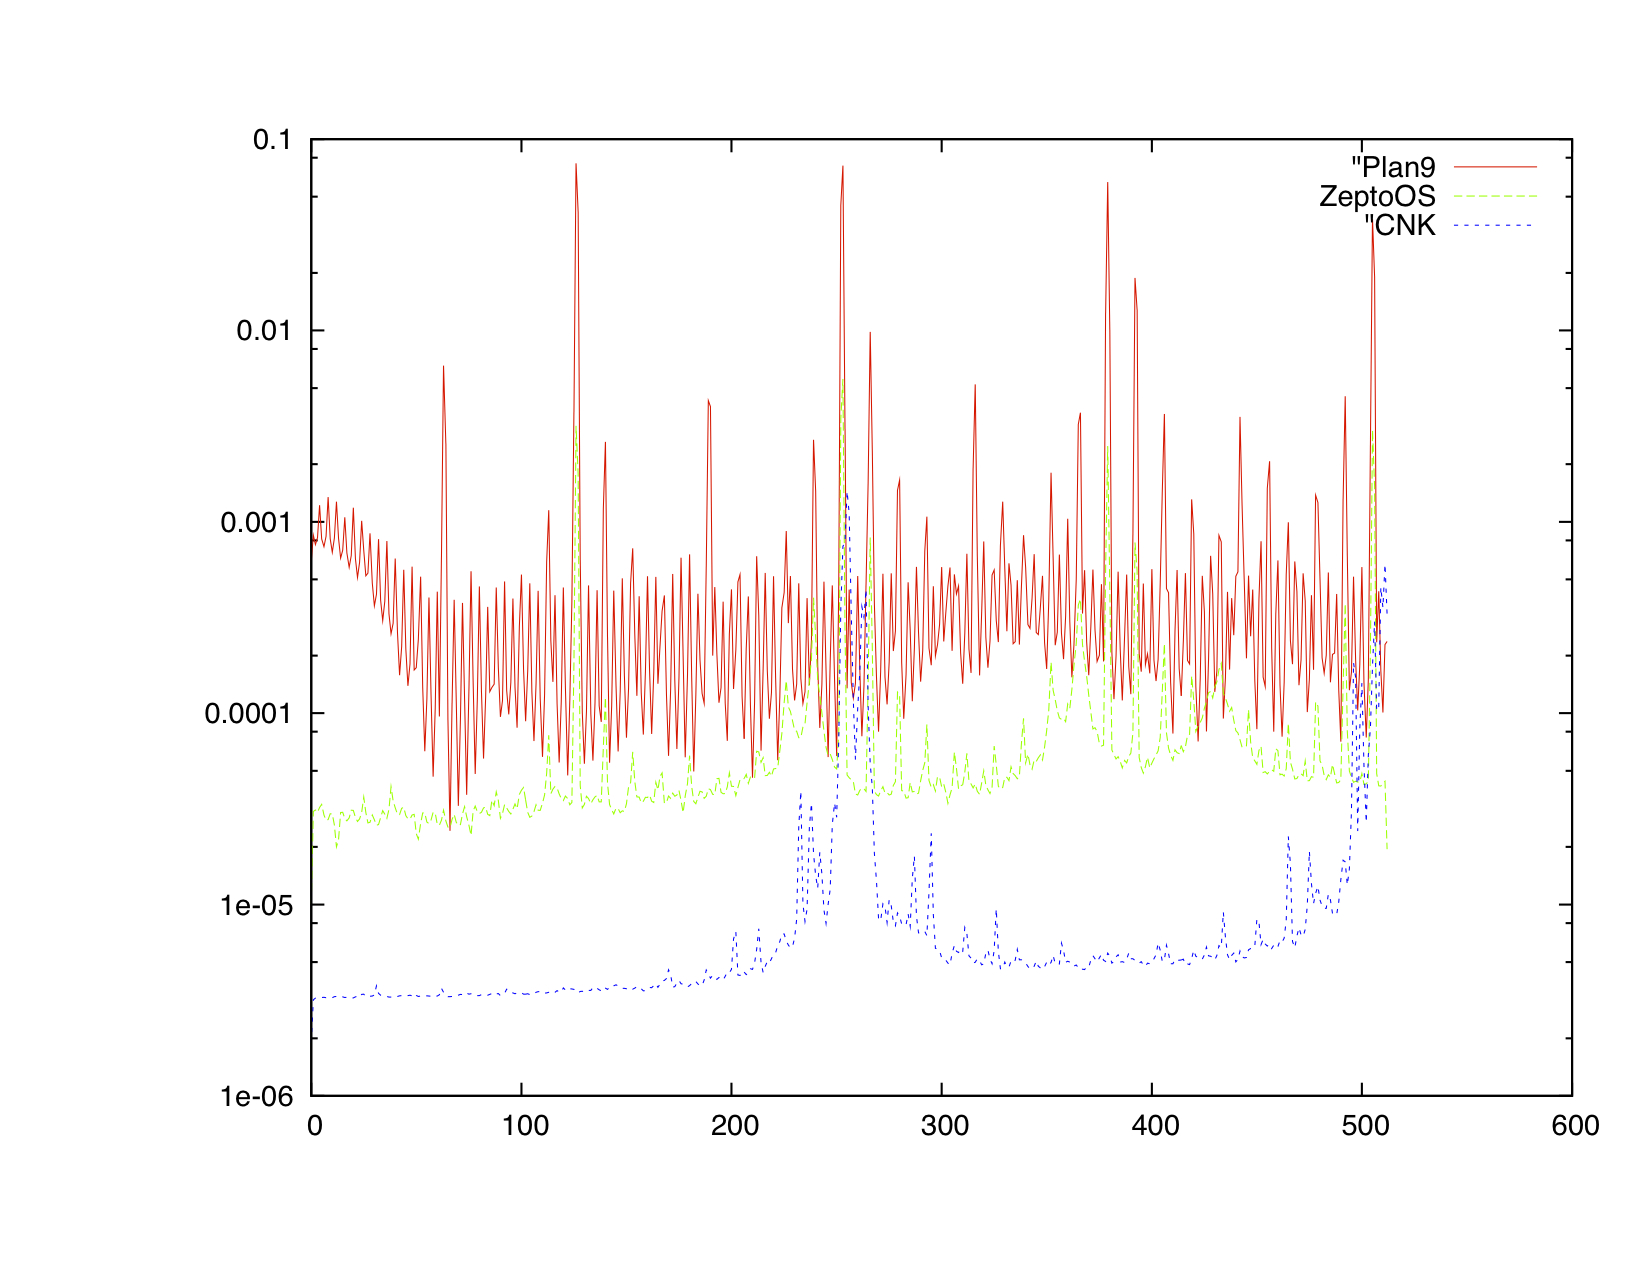
\includegraphics[width=5in]{spectrum.jpg}
\caption{{\bf Power Spectral Density for the three operating systems, Frequency in HZ on the x axis
and unit-less amplitude on the Y axis.}}
\label{psd}
\end{center}
\end{figure}

The graph shows that CNK has a better noise figure than either of its two
more general purpose competitors. It is also possible to see
the frequencies at which noise spikes occur. In fact, an earlier version 
of this chart revealed a very distinct noise spike at 30 HZ. which we 
eliminated. Finally, it is easy to see that, while there is an apparent similarity in the time
domain between CNK and ZeptoOS noise,they are not at all similar in the
frequency domain. One can not simply look at raw data graphs and 
reveal all the hidden information. 

FTQ allows us to quantitatively measure and analyze noise, using standard 
signal processing techniques. Spectral components of noise can be measured, 
traced back to their source, and eliminated. 


\chapter{Operating Systems Developments}
\section{Plan 9 Port to Blue Gene /L and /P}
\subsection{Large Pages}
Blue Gene   processors use software-loaded TLBs. A TLB manages the virtual to physical mapping for a single page, which 
in both Linux and Plan~9 is 4096 bytes. The processors support more than just one page size, in multiples of 4, from 1024 bytes to 1 Gbyte (with a few sizes missing). 
The CNK 
features 1 Mbyte TLBs, and benefits from reduced TLB fault interrupts. 

We extended Plan~9 to support larger TLBs. In order to measure the improvement we used the strid3 benchmark
\begin{figure}[h]
\begin{center}
 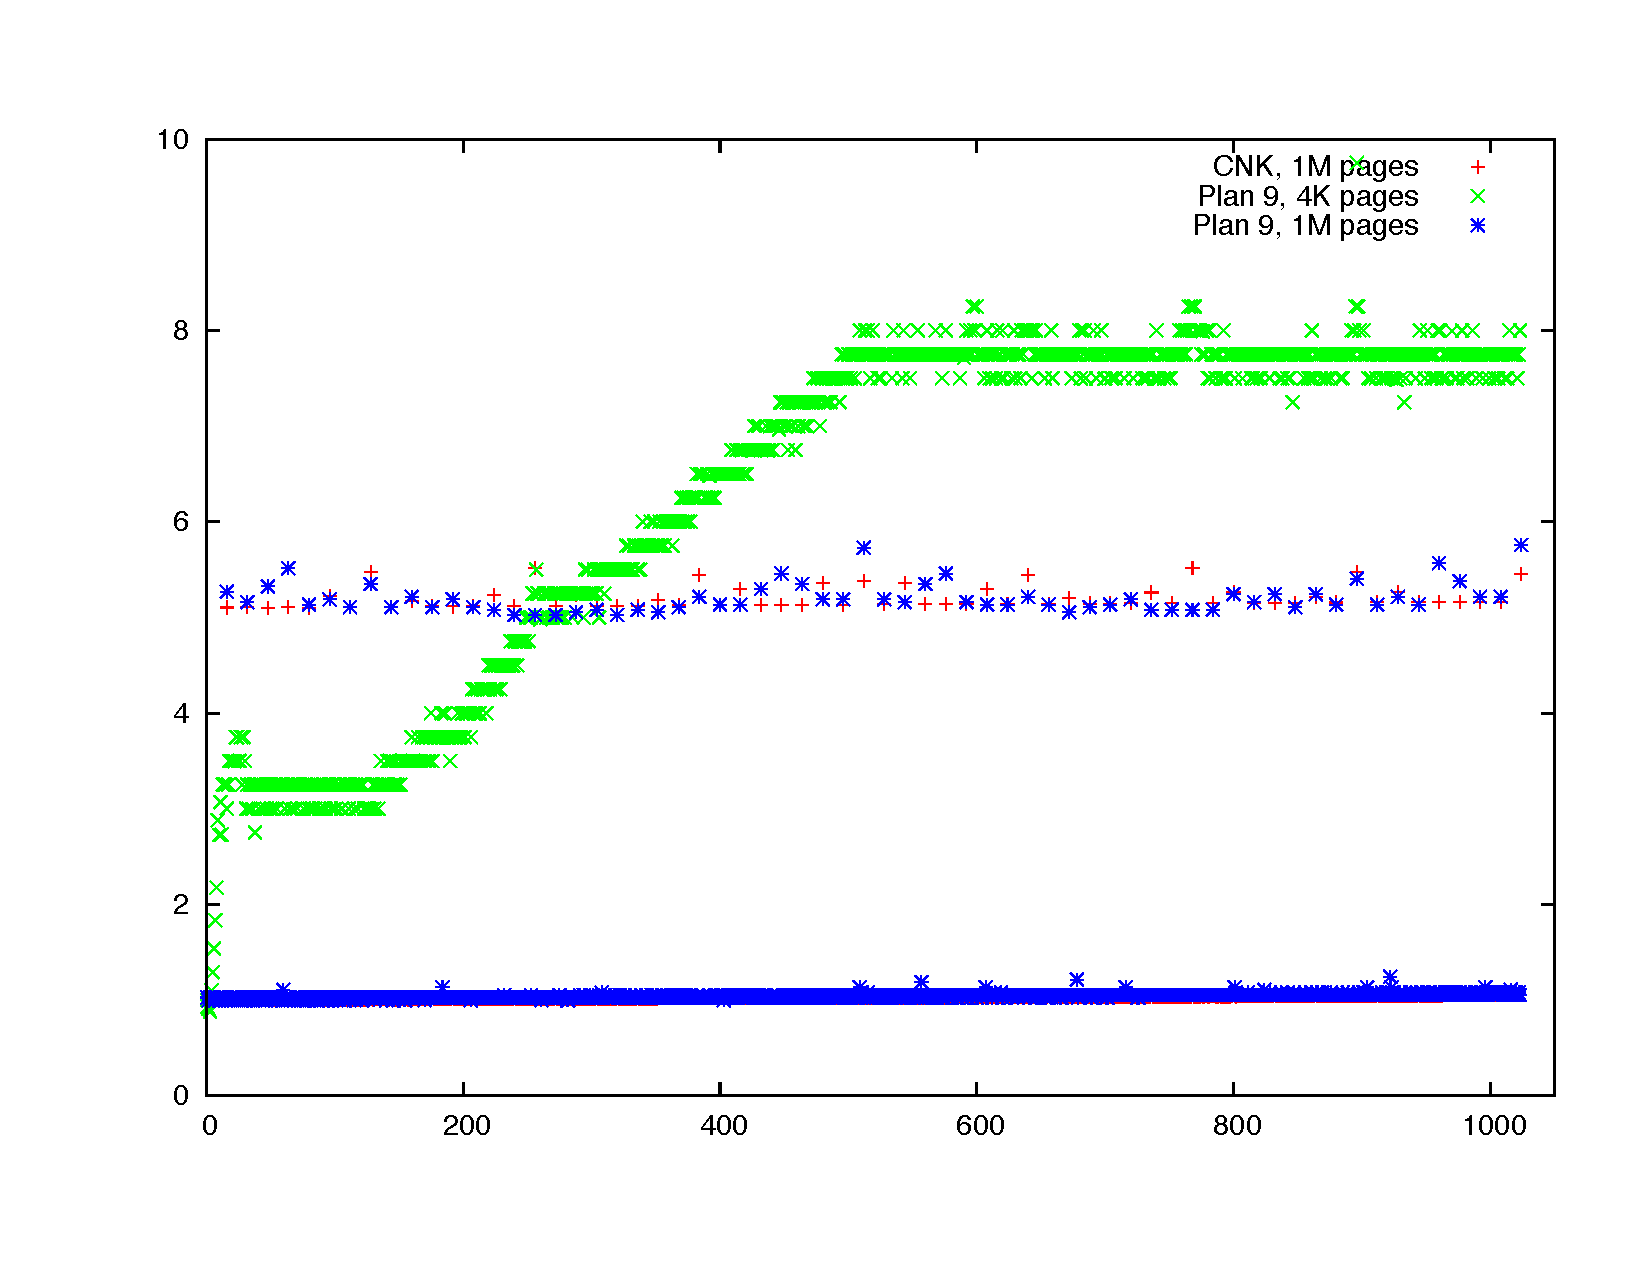
\includegraphics[width=4in]{strid3.pdf}
 \caption{{\bf Result of running strid3 on CNK, Plan 9, and Plan 9 with 1 MByte pages. }}
\label{strid3}
\end{center}
\end{figure}
to show the impact of TLB size upon an application. Shown in Figure \ref{strid3} is the result. Plan~9 is 
eight times slower than the CNK when 4096 byte pages are used. With one Mbyte pages in Plan~9, its 
performance is identical to the CNK. 
The change to Plan~9 to support the larger pages amounted to less than 30 lines of code\cite{DBLP:journals/ife/MinnichM09}. 

\section{Currying and Process-private system calls}
Extensive measurement of the kernel, using the tool developed and described in \cite{plan9trace}, showed
that for read and write system calls a great deal of overhead was repeated for each iteration of the 
call. Two of the biggest overheads are validation of the file descriptor and the read/write pointer and 
length validation. We also found in most cases that the pointers are being reused for each call: it is extremely rare for these parameters to be wrong, yet programs pay the full overhead for checking them 
each time. For the Blue Gene global barrier device, the overhead for the system call was 3.529 microseconds. 

In \cite{currying} we describe the possible approaches to resolving this problem. We developed two 
several extensions to Plan~9 that allowed the kernel to Curry the arguments to the read and write
system calls. The result: the file descriptor and point/length information is checked once, and the
result stored in a cache held in the proc struct (per-process information) in the kernel. The per-process structure is 
also extended with a private system call table. When the process makes a private system
call, all the standard checking is skipped and the cached values are used instead. This 
new system call path resulted in a 5-fold reduction in overhead, to 729 nanoseconds. 

The Currying and per-process system calls together form a new type of interface to operating system
kernels. 

\subsection{Shared Heap}
Shared data is an important part of HPC applications. 

\section{File Systems}
\subsection{Compute Node Caches}
\section{New network communications models}
\subsection{Active Message Support}
\subsection{What are we calling Charles stuff?}
\section{Kittyhawk Kernels and VMM}

Supercomputers and clouds both strive to make a large number of 
computing cores available for computation. 
However, current cloud infrastructure does not yield the performance 
sought by many scientific applications. A source of the performance 
loss comes from virtualization and virtualization of the network in 
particular. 
Project Kittyhawk~\cite{kh-sciencecloud} was an undertaking at IBM Research 
to explore the use of a hybrid supercomputer software infrastructure
on top of a BlueGene/P which allows direct hardware access to the 
communication hardware for the necessary components while providing 
the standard elastic cloud infrastructure for other components.

Beyond the enabling infrastructure for cloud provisioning and dynamic
boot of multiple images across compute nodes within a single BG/P
allocation, the Kittyhawk team also ported a Linux compute node
implementation complete with an Ethernet interface to the high-performance
collective and torus networks~\cite{kh-systemsjournal}.  
This allowed Linux applications to run unmodified om Blue Gene compute 
nodes without incurring the performance 
overhead of reflecting sockets and I/O operations thorugh user space
helpers as in ZeptoOS.  It also enabled more conventional storage solutions
including SAN and NAS to be extended into the compute node network for
I/O intensive solutions.  While the Kittyhawk Linux kernel provided this
Ethernet interface, it also provided an API allowing the allocation of
torus channels directly to high performance applications which knew how to
interact with them allowing even greater degrees of performance and flexibility.
These allocated application channels co-existed with the kernel-space channels
providing a good hybrid trade off between system provided networking and
OS bypass.

The Kittyhawk environment was not limited to Linux kernel targets.  
It also supported execution of the L4 microkernel operating system.  
In addition to providing an alternative execution platform for applications,
the L4 Kittyhawk port also supported a virtual machine monitor which could
be used to further virtualize the BG/P nodes and network providing additional
protection in cloud deployment environments.

The Kittyhawk infrastructure, the linux kernel patches, and the L4 kernel
and virtual machine monitor have all been released as open source and are
available from http://kittyhawk.bu.edu.

\chapter{Run Time Developments}
Developing runtimes for processes on Plan~9 was challenging, because we did not opt for the 
traditional HPC approach of placing device drivers in user level libraries. From the beginning of this 
project, we had decided to have the kernel control communications and  
resource management tasks that have 
been relegated to user level runtimes for decades. Returning control of these tasks to  the kernel
makes the HPC resource available to a much wider set of applications than just MPI programs. On 
many traditional HPC systems, high performance networks are not even visible to non-MPI 
applications. On Plan~9 on BG/P, even the command shell has access to the fastest networks: hence
it is 
possible to run a shell pipeline between compute nodes, without rewriting all the 
programs involved to use MPI. Parallel programs become more portable, and much easier to 
write and use. 

Removing device drivers from libraries removed all the attendant complexity from those libraries; 
many user-level libraries have more complex code than the Plan~9 kernel, and even the smallest 
of those libraries is larger than our kernel. Our limited-function MPI supports many MPI applications 
in less than 5000 lines.

User-level runtimes are not without their advantages. Most MPI libraries are thread-safe, and 
incorporate an activity scheduler that can choose activities with very low overhead. Because the 
device driver is contained in the process, pointers to data are valid for all the operations the runtime 
performs, including setting up DMA. There is no need to translate addresses, and 
on a simple system like Blue Gene, there is no need for complex page pinning software. 
These MPI runtimes in essence create a single-address-space operating system, complete with drivers 
and scheduling, that is "booted" by the host operating system and then left to run in control of the
node. Again, the advantages of the runtime include the implementation  of system call functionality 
with function calls; and a single
address space, with the attendant elimination of address translations and page faults and 
elimination of unnecessary copies. 

Leaving device drivers in the kernel requires reduced overhead in some areas. 
A system call takes 1-2 microseconds, on average; this time must be 
reduced when latency-sensitive operations take place. User-level 
addresses must be mapped into the kernel address space. In interrupt handlers, user-level 
memory is not easily accessed in Plan~9, since interrupt handlers have no user context. 

In this section we describe the research we have undertaken to address these needs. 

\section{Currying and Process-private system calls}
Extensive measurement of the kernel, using the tool developed and described in \cite{plan9trace}, showed
that for read and write system calls a great deal of overhead was repeated for each iteration of the 
call. Two of the biggest overheads are validation of the file descriptor and the read/write pointer and 
length validation. We also found in most cases that the pointers are being reused for each call: it is extremely rare for these parameters to be wrong, yet programs pay the full overhead for checking them 
each time. For the Blue Gene global barrier device, the overhead for the system call was 3.529 microseconds. 

In \cite{currying} we describe the possible approaches to resolving this problem. We developed two 
several extensions to Plan~9 that allowed the kernel to Curry the arguments to the read and write
system calls. The result: the file descriptor and point/length information is checked once, and the
result stored in a cache held in the proc struct (per-process information) in the kernel. The per-process structure is 
also extended with a private system call table. When the process makes a private system
call, all the standard checking is skipped and the cached values are used instead. This 
new system call path resulted in a 5-fold reduction in overhead, to 729 nanoseconds. 

The Currying and per-process system calls together form a new type of interface to operating system
kernels. 


\section{XCPU^3}
\section{UEM}
\section{PUSH}

\chapter{Infrastructure Developments}
\section{Blue Gene Debug File System}
\section{nompirun}
\section{Kittyhawk Cloud Provisioning}


\chapter{NIX}

NIX is an operating system designed for manycore CPUs in which not 
all cores are capable of running an operating system. Examples of such 
systems abound, most recently in the various GPU systems. While most 
heterogeneous systems treat the non-OS cores as a subordinate system, 
in NIX they are treated as peers (or even superiors) of the 
OS cores. 
Many  additional features of NIX were created based on what we learned from 
the RWK and HARE projects. 

NIX
features a heterogeneous CPU model and can use a shared address space
if it is available. 
NIX partitions cores by function: Timesharing Cores, or
TCs; Application Cores, or ACs; and Kernel Cores, or KCs.  One or more
TC runs traditional applications.  KCs are optional, running kernel
functions on demand.  ACs are also optional, devoted to running an
application with no interrupts; not even clock interrupts.  Unlike
traditional kernels, functions are not static: the number of TCs, KCs,
and ACs can change as needed.  Also unlike traditional
systems, applications can communicate by sending messages to the TC
kernel, instead of system call traps.  These messages are "active"
taking advantage of the shared-memory nature of manycore CPUs to pass
pointers to data and code to coordinate cores.

NIX has transparent support for a near-unlimited range of page sizes. 
On the 64-bit x86 family, for example, NIX supports 2 MiB and 1 GiB pages. 
Support for 1 GiB pages is crucial to performance: on one popular 
graph application we measured a 2x speedup when 1 GiB pages were used 
instead of 2 MiB pages. 
The implementation allows for virtual pages, e.g., one could 
provide 16KiB pages that are a concatenation of physical 4 KiB pages. 
These virtual pages would allow us to reduce the number of page 
faults an application causes, although they would not reduce 
TLB pressure. 

NIX gives us the best of many worlds. Applications can own a core, 
and will not even be preempted by a clock tick, as they are even 
on Light Weight Kernels today. At the same time, the full capability 
of a general purpose operating system is available on core nearby. 
We feel that NIX represents the shape of future operating systems
on manycore systems that are being built now. 

Further information on NIX can be found in Appendis A. The source 
code is available at https://code.google.com/p/nix-os. 

\chapter{Future Work}
%Over the period of these two projects, we have shown that with appropriate 
%modifications, general purpose operating systems can be used for HPC computers. 
%We have developed tools that show the quantitative benefit of these 
%This experience confirms the experience of industry. 
This research has suggested a number of new directions for HPC. 
\begin{itemize}
\item New operating systems that step outside the stale Light-Weight Kernel/General Kernel
argument. We have shown that one such kernel, NIX, can support the desirable attributes of both
and even outperform LWKs at the things they do best. 
\item Network IO can and should be done in the kernel, and future research should 
work out the API. OS Bypass should be bypassed. 
\item Network software that does not assume a perfect network needs to be created and put into use.
This change in turn will allow innovation to occur in 
HPC hardware. 
\item HPC hardware needs to change so that it can provide near-perfect
information about failures, but not nodes that never fail. Software 
can handle faults in a far more flexible manner than hardware. 
\item File systems must change to make explicit use of hierarchy. The ratio of Compute Nodes to IO Nodes should not be 
statically defined by wires, as it is today, but defined by the needs of the application, and hence flexible. 
\end{itemize}

\chapter{Conclusions}

While no commercial HPC vendor is using Plan~9, they are using much of the other software we developed, 
including the 64-bit compiler toolchain, FTQ, and NIX. 
There are other lessons learned: 
\begin{itemize}
\item OS bypass is not required for good network performance. ``Conventional knowledge
bypass'' is much more important: if we can get runtime libraries to accomodate 
such concepts as a shared heap address space, we can reduce runtime and OS 
complexity and remove OS bypass for the most part. 
\item The idea of quantitative measurement of OS noise was controversial when we first proposed it in 2004. 
In fact, there is a wealth of signal processing software and knowledge that can be applied to HPC. We need
to move beyond qualitative descriptions to quantitative measurements. Adjectives should be avoided
when numbers can be supplied. 
\item Users want a Unix-like API, even on systems like Blue Gene which do not run Unix on all nodes. 
Key requirements such as sockets, dynamic libraries, and a reasonably standard file system
interface can not be waved away. Light Weight Kernels that fail to provide these services
will either change (as did the CNK) or be abandoned by the vendor (as was Catamount). 
\item As pointed out above, ``Thus, for reliable communication, the hardware level flow-control is neither necessary nor sufficient, 
and flow-control must be added somewhere in the multiplexing software stack.'' Communications networks
on future architectures could be made simpler, faster, more reliable, and lower power by taking 
this fact into account. 
\item We need to move beyond simply gluing hardware interfaces into existing kernel designs in non-optimal ways. 
One of the worst examples of this tendency can be seen in the Linux drivers for HPC networks: they all emulate an Ethernet. 
This emulation results in ineffeciencies and poor software structure: 
the Jaguar system, for example, has 30,000 hardwired ARP-table entries 
{\em on each node} so that the TCP/IP address in $[x,y,z]$ form 
can be mapped to an Ethernet address in $[x,y,z]$ form. 
Ethernet interfaces are for Ethernet networks. There is no need to have a network interface for an
HPC network 
emulate an Ethernet, as it does on Compute Node Linux on the Cray or 
ZeptoOS on BG/P. 
\end{itemize}

This work was done as part of the FAST-OS program and its successor. 
The ground was prepared for the FAST-OS programs in a series of meetings held in
the eary 2000s. One of the PIs earliest talks dates from 2002. In 2003, we made
the following arguments: 
\begin{itemize}
\item Linux is fun and working now; enjoy it
\item Linux is not forever
\item Some fundamental properties of the Unix model have fatal flaws
\item We are entering a period of “architecture flux” 
\item We need diversity in OS research now to prepare for new, strange machines
\item DOE can succeed in creating a successful, diverse OS research community
\end{itemize}

We might ask: is any of this less true now that our community is faced with 
the challenge of scaling parallelism up 1000-fold? We would argue that 
the problem is even worse. While this program may have had successes, in some 
sense the community is 
still plowing the same ruts. The extant machines still largely run Linux, and the 
problems we predicted in 2003 (for the 2012 timeframe) are starting to 
come to pass: with each new version, Linux gets just a bit slower, as it grows in size 
and complexity and the processors do not get any faster. As we stated in 2003, 
``At some point, like all other OSes, it is [Linux] going to fall over''. 
Several large companies, in private conversation, have told the PI that one of the
biggest management headaches they have is dealing with the increasing complexity of 
the Linux kernel, version to version, as it gains more features and bulk.  

Did FAST-OS succeed? That is a harder question. In the sense of industry impact, we 
clearly had great success. In the sense of building a vibrant community of OS researchers
in DOE, we had some success; there is very good OS work going on at Argonne, Oak Ridge, 
and Sandia, and on a smaller scale, at other Labs. 

Those are hard-won gains, and maintaining them 
will not be easy: OS research continues to come under 
pressure for both budget reasons and 
from those who believe that industry will just supply an OS as a turnkey 
answer, in spite of all historical evidence to the contrary. No standard OS has ever worked
for the large scale without substantial measurement and change. 

Further, the challenges 
in the worlds of Google, Amazon, and Facebook are now much bigger 
and freer of past constraints: just this year Google announced 
the Exacycle initiative, and is delivering one billion core
hours for researchers. 
Further, the scale of the commercial world's file storage problems now dwarfs 
anything that is facing DOE. Hiring and keeping people at 
DOE Labs is becoming ever more challenging, absent support for 
new and novel approaches to DOE problems. People are not excited
by the idea of spending the next 10 years of their career supporting 
the legacy software produced over the last quarter century. 

DOE needs to build on the success of these programs by continuing
to fund new, innovative research that will 
help vendors set new directions. 
At the same time, DOE Labs should almost never be in the business of 
providing production software; 
nor should commercial uptake of every last bit of research software
be the standard 
by which success is measured. 
Failure should always be an option. If there are no failures, 
then the research is not nearly aggressive enough. 

When FAST-OS started, the discussion was whether the DOE Labs would have any OS 
knowledge or capability left by the end of the decade. FAST-OS and its successor
program created a culture of competency in the DOE Labs and attracted some very 
capable commercial and research partners  from outside the labs. 
In the end, we count this research, 
and the larger program that funded it, as a success. Whether
the gains we have made will be maintained is a question that can only 
be answered at the end of {\em this} decade. 

%\bibliographystyle{abbrvnat} 
\bibliographystyle{plain}

\bibliography{all}

\appendix
\appendixpage
\section*{NIX}
This document will appear in Bell Labs Technical Journal and was the subject
of a talk at a Bell Labs Technical Conference in Antwerp, Belgium, Oct. 2011. 
\newpage
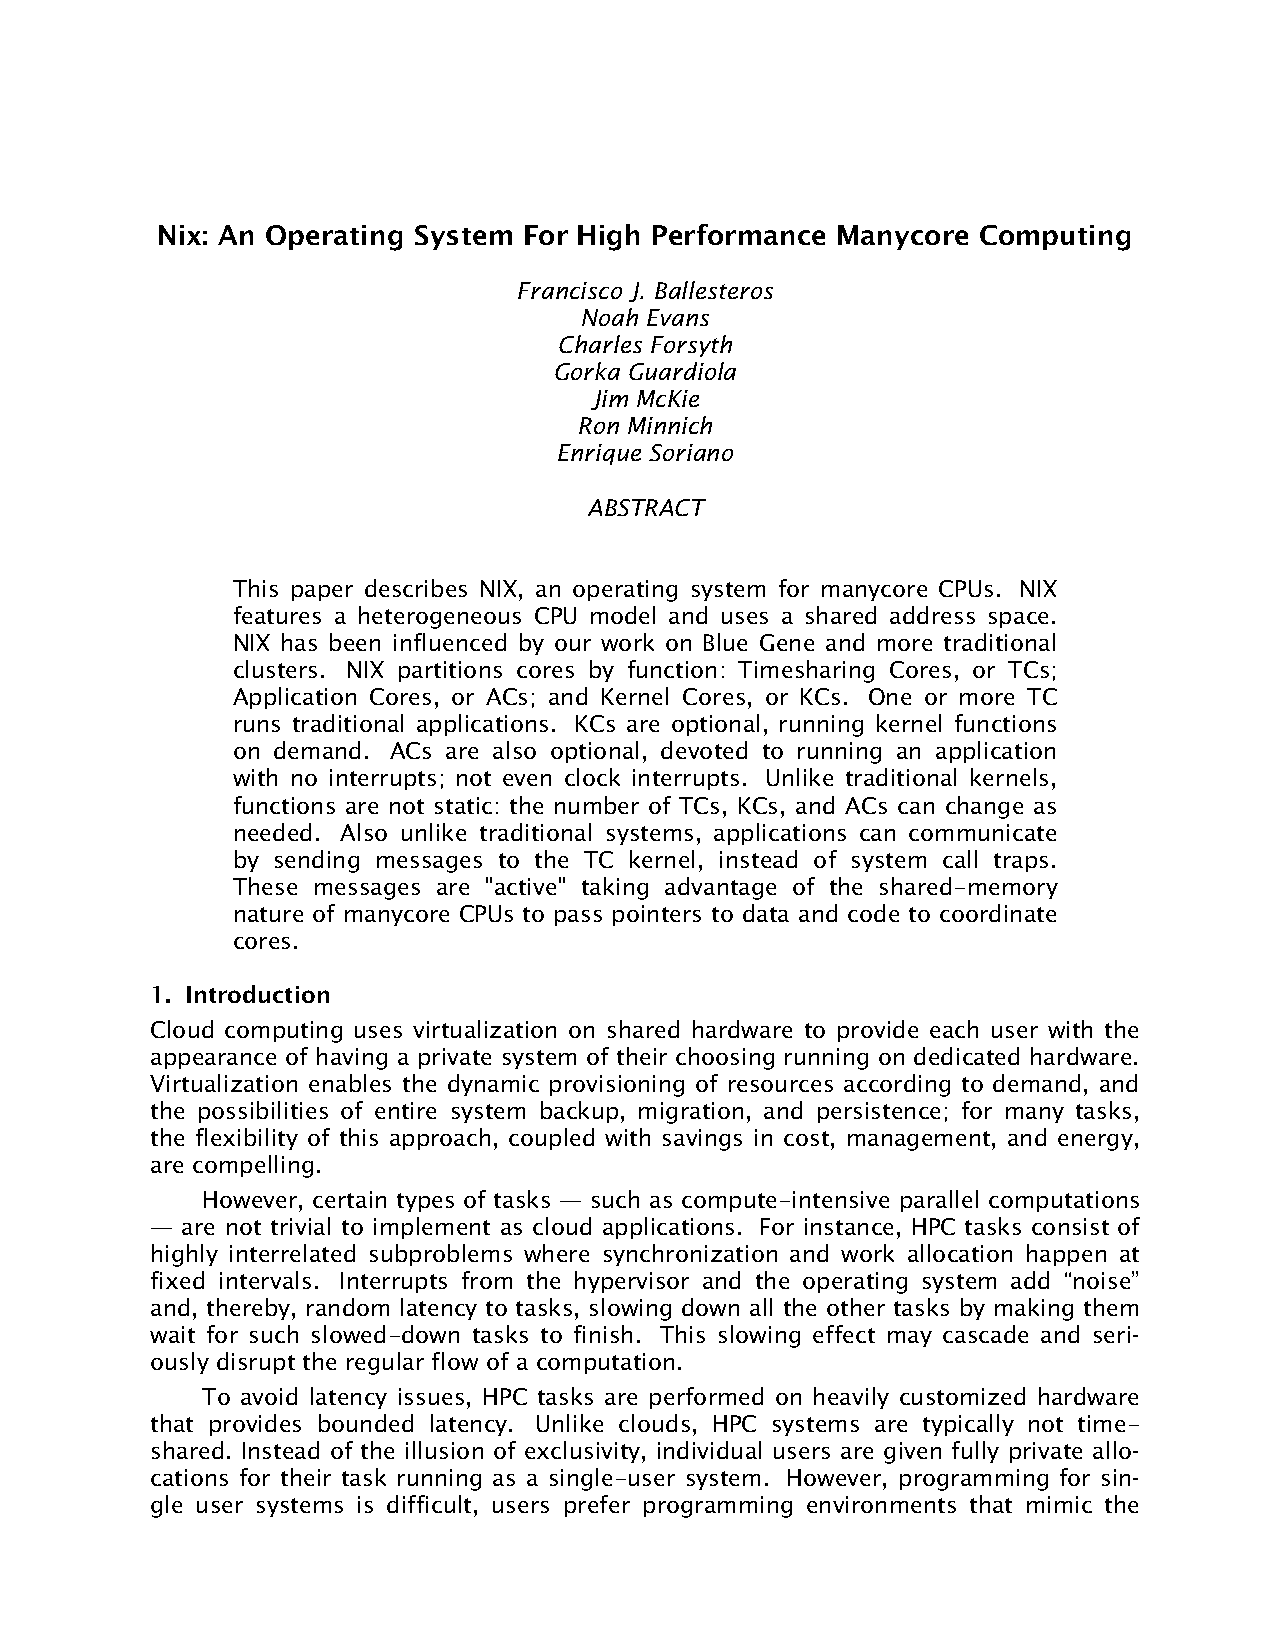
\includepdf[pages=-]{bltj.pdf}

\addappheadtotoc
\end{document}
